%        File: pnas1.tex
%     Created: Wed Apr 30 04:00 pm 2014 E
% Last Change: Wed Apr 30 04:00 pm 2014 E
%
\documentclass[a4paper]{report}
\usepackage[hmargin=2cm,vmargin=2cm]{geometry}
\usepackage{scrextend}
\usepackage{graphicx}

\usepackage{amsmath}
\usepackage{amssymb}
\usepackage{mathrsfs}
\usepackage{gensymb}
\usepackage{algorithm2e}
\usepackage{amsthm}

\newtheorem*{mydef}{Definition}

\usepackage{cite}

\usepackage{framed, color}
\usepackage{soul}
\usepackage[colorlinks=false, urlcolor=blue]{hyperref}
\usepackage{dcolumn}
\usepackage{multirow}
\usepackage{booktabs}
\newcolumntype{d}{D{.}{.}{4.0}}
\newcolumntype{s}{D{.}{.}{1.4}}

\newcommand{\td}[1]{{\color{blu}\hl{TODO: #1}}}

\definecolor{shadecolor}{rgb}{.93,.93,.93}
\definecolor{blu}{rgb}{0,0,1}
\setlength{\parindent}{0cm}
\setlength{\parskip}{4mm plus1mm minus1mm}


\title{Inter-task effects induce bias in crowdsourcing}
\author{Edward Newell, Derek Ruths}

\parindent0pt \parskip8pt

\begin{document}
\maketitle
\section*{Abstract}
Microtask platforms like Amazon Mechanical Turk provide a cheap and fast means
to engage participants for scientific reasearch.  
Workers on such platforms prefer to work on batches of tasks of the same 
type[***], so we investigate the potential for the content of earlier tasks 
to influence worker performance in later tasks, which we call ``inter-task'' 
effects.  
Existing research investigates the impact of various design factors, such as 
``framing'', on the quality of crowdsourced content, but does not, to 
our knowledge, address inter-task effects.  
We employ a canonical image-labeling task on the Amazon Mechanical Turk 
platform, to measure both inter-task and framing effects, in terms of their 
impact to the content and specificity of the labels workers provide.
We also introduce an algorithmic definition of priming, which measures the 
worst-case bias that priming effects introduce into crowdsourced content.
We find that inter-task effects produce a much stronger impact than framing, 
and find that our algorithmic definition yields a powerful, generalized measure
for priming effects when combined with machine learning algorithms.


\section*{Significance Statement}
\section*{Introduction}

Microtask crowdsourcing platforms like Amazon Mechanical Turk (AMT) make it 
possible to submit batches of small tasks to a large pool of human workers, 
who do the tasks for fun, a sense of purpose, and remuneration 
\cite{kazai2013analysis, Antin20122925}.  
Originally used to distribute clerical work, these platforms 
increasingly serve as a fast and cheap means to engage experimental 
participants and manually annotate datasets in a research 
setting \cite{snow2008cheap}.  
Tasks involving qualitative
judgment (e.g. flagging inappropriate images), natural language annotation,
and object recognition are commonplace, since it is difficult to achieve 
comparable performance using only computers \cite{yuen2011survey}.
%Generally the worker is first given some orientation to the task, and then 
%performs the task repeatedly (e.g. label several images, one after 
%the other).

Such platforms make human cognition a fluid resource: it is available 
on demand in small units, with low transaction 
cost, from anywhere via the 
Internet\footnote{\href{http://mturk.com}{http://mturk.com}}.
The task requester can 
interact with the platform like a compute server, seamlessly 
integrating human and machine computation.  Researchers have put forward the 
term HPU (Human co-Processing Unit)\footnote{We acknowledge the irony of this 
term: the original meaning of `computer' was a person who performs 
computations, its reference to machines being a personification brought into 
usage in the late 1800s\cite{Dictionary:hl}.}, viewing the introduction of 
microtask platforms as a new computing architecture
\cite{5543192}.  

Here, we highlight an important way in which HPUs differ from CPUs, with 
serious implications for the design of tasks.  It is well known that people 
are subject to priming effects 
\cite{BJOP:BJOP1796, No2007, beller1971priming} and, in particular, task-repetition effects
\cite{Gass1999549, sohn2001task}.  
We investigate the effect that previously completed tasks have on workers'
responses during subsequent ones. We call such effects 
\textit{inter-task priming}.  Inter-task priming would amount to a kind of
\textit{hysteresis}, meaning that HPU output is not only a function of the 
current input, but also of the history of inputs.

There has been considerable investigation into the factors that affect HPU 
output on crowdsourced microtask platforms.  Studies have shown that 
there is a great deal of variance in worker attention and 
accuracy \cite{kazai2013analysis}.  Factors that affect the quality of HPU 
output include level of pay\cite{kazai2013analysis}, 
training\cite{le2010ensuring}, screening workers\cite{paolacci2010running}, 
and user-interface design
\cite{Finnerty2013}.  Research has also investigated \textit{framing}, 
by testing the effects of disclosing the role of a task within the 
context of a study \cite{Kinnaird2012281}, and disclosing the ultimate 
purpose of that study \cite{chandler2013breaking}.  However, to our knowledge, 
no study has investigated the effects of inter-task priming.

To characterize the effects of inter-task priming, we present a novel  
\textit{algorithmic definition of priming}, along with a general method 
for measuring priming effects using machine learning algorithms.  
Existing work on priming effects focuses on the internal psychological 
mechanisms of priming[***], but here we are interested in how the treatment of 
workers can impact an application of human computation. This leads us to 
quantify priming in terms of the algorithmic distinguishability of priming
treatments.

In the present work, we investigate inter-task priming using image-labeling 
tasks on the AMT platform.  
(***why we are using image labeling as prototypical task***) 
Each worker is required to label ten images 
featuring 
food and culture.  We regard these images as being made up of an 
\textit{initial} and \textit{final set}, but, crucially, there is no
distinction made between these sets, nor any interruption in the flow of tasks 
from the view of the worker.
Each worker is randomly assigned one of three initial sets, but the final set
of images is always the same.  We analyze the effect that the assignment of 
initial set has on workers' attribution of labels to the final set.  We 
measure effects using our novel approach, as well as looking for changes in 
the content of labels and label specificity based on an ontology we 
developed for that purpose.

As a point of comparison, we subject some groups of workers to a kind of
\textit{framing}: we disclose a fictitious, semantically-loaded name for 
requester funding the tasks.
The names were chosen to suggest the requester's interest in 
a specific aspect of the image content.  One might reasonably expect that this 
would orient workers to provide a greater quantity and specificity of labels 
which relate to this ``preferred'' content[***].

Surprisingly, we find that inter-task effects on label orientation and 
specificity are much stronger than those brought about by framing tasks with a 
funder name.  Our results show that initial tasks can introduce significant 
bias in subsequent worker labeling.  Interestingly, we find that inter-task
effects can be used to induce greater specificity.  Our results suggest that
workers attribute more specific labels when labeling a series of images that
that are more similar to one another.  This suggests that careful 
consideration should be given to the bundling of tasks when designing a study 
using a microtask platform.

Our analysis also highlights important advantages of our novel definition of 
priming.  Our approach relies on no prior knowledge about the nature
of the task task whatsoever.  In contrast, we also sought to detect priming
based on its direct effects on label content and specificity, implicitly
drawing on prior knowledge about the images and label semantics.
Remarkably, while being more general, our novel approach was also more 
sensitive.  This suggests that our measurement approach could be applied in 
cases where one does not \emph{a priori} know whether any priming has occurred, 
nor what the effects might be.

\subsection*{An algorithmic definition of priming}

In psychology, the effects of priming are usually measured in terms of a 
change in the  
speed or accuracy of responses in a task, or in the ability to recognize a 
stimulus object (e.g. a spoken word or an image) when the object is noisier, 
fainter, or briefer [***].  Methods are also employed to measure processes
in the brain of the participant, such as by fMRI[***].  These approaches are 
well-suited to studying the underlying psychological mechanisms at work.

Our purpose is different: we are interested in assessing the ramifications
that priming of HPUs could have on the applications to which they are employed.
This influences the approach we take to measurement in two ways.  First, we 
switch from focusing on the internal mechanisms of HPUs to focusing strictly 
on the HPU outputs.  Second, we cannot \textit{a priori} know the 
application for which HPUs are being employed, but we would like to measure 
any effects that could in principle impact the application.  These 
considerations motivate us to define priming effects in terms of the 
algorithmic distinguishability of primed output.

One difficulty in constructing a definition of priming is that there would 
appear to be no defensible notion of a ``neutral'' or ``unprimed state''.  A 
participant 
always approaches a task in \textit{some} state of mind.  If no priming 
condition is applied, then the participant is simply primed by her
exposures prior to the experiment, which cannot be known by the experimenter.  
While arguments can surely be made that one treatment or another is 
\textit{more} 
``neutral'', we refrain from proposing a canonical ``null priming treatment''. 
Instead, we define priming relatively, and speak of one treatment being 
\textit{differently primed} from another.

A definition of priming must also consider that the effects of priming will
manifest differently depending on the task that participants perform 
subsequent to priming:  two priming treatments that
produce markedly different output for one task might be 
indistinguishable under another task.  Thus, we define priming
with respect to a task.

A final factor to consider is that people will always differ in their initial
knowledge, specific aptitudes, and in many other intrinsic aspects.  Moreover,
priming may not be ``complete'', in the sense that people's experiences before
priming may continue to have residual effects.  Therefore, we define priming 
in relation to populations, which we regard as having stable distributions of
such latent attributes.

To set up the definition, when a population of people $\mathcal{J}$ performs
a task $\mathcal{T}$ thus producing a population of task-outputs $\mathcal{L}$,
we will write $\mathcal{T}(\mathcal{J}) = \mathcal{L}$.

\vspace{2mm}
\begin{mydef}
	\upshape
	Two mutually exclusive populations of people, $\mathcal{P}_0$ and 
	$\mathcal{P}_1$, are uniformly and randomly subsampled from an initial 
	population $\mathcal{P}$, are exposed to (possibly) different priming 
	treatments, and then perform a task $\mathcal{T}$, 
	producing task-outputs $\mathcal{T}(\mathcal{P}_0)$ and 
	$\mathcal{T}(\mathcal{P}_1)$.
	These populations are subsampled, producing 
	$P_0 \subset \mathcal{P}_0$ and
	$P_1 \subset \mathcal{P}_1$. A uniform, random bit is chosen, 
	$b\in _R \{0,1\}$, and a single worker $p$ is uniformly and randomly 
	sampled from 
	$\mathcal{P}_b \setminus P_b$.
	We say that $\mathcal{P}_0$ and $\mathcal{P}_1$ 
	\emph{differ in priming by a degree at least $\theta$},
	if there exists a \emph{distinguisher algorithm} $\mathcal{A}$ that takes as input 
	$\langle\mathcal{T}(J)$, $\mathcal{T}(K)$, $\mathcal{T}(\{p\})\rangle$
	and outputs a guess for $b$ with accuracy $\frac{1+\theta}{2}$.  
\end{mydef}

In the language of computer science, $\mathcal{A}$ is a classifier performing
a binary classification.  The measure $\theta$ can range between 0 and 1, and 
indicates how much better the performance of the best possible classifier is 
compared to a random guess. We intentionally leave the details of 
$\mathcal{A}$ unrestricted because $\theta$ should depend on the potential 
for two populations to be distinguished, based on their inherent differences, 
rather than on the performance of a particular classifier.

In practice, some particular classifier $\mathcal{C}$ must be used and a 
statistical estimate of its performance $\hat{\theta}_\mathcal{C}$ obtained. 
$\hat{\theta}_\mathcal{C}$ acts as a lower bound for the 
theoretical value $\theta$ from the definition, because there might 
exist some other classifier $\mathcal{C}'$ with 
$\hat{\theta}_\mathcal{C'}>\hat{\theta}_\mathcal{C}$.
Here, we use a Naive Bayes classifier because it simple and performs well 
across a broad range of classification tasks[***].

To interpret $\hat{\theta}_\mathcal{C}$, imagine that some choice is to be
made between two options on the basis of worker outputs (e.g. whether or not 
to flag an image as inappropriate). Any such binary choice has a formal 
structure of a trained classifier (i.e. a distinguisher which discards the 
first two inputs). This means that $\hat{\theta}_\mathcal{C}$ estimates a 
lower bound for the worst-case bias introduced in such a binary decision when 
one failed to control for priming effects.

\subsection*{Experimental Setup}
\begin{table}[t]
\centering
	\begin{tabular}{ l  l  l }
		\hline                       
		Treatment & Funder & Priming Image Set	\\ 
		\hline                       
		$\textsc{ambg}$ & None & Ambiguous\\
		$\textsc{cult}_{img}$ & None & Cultural\\
		$\textsc{cult}_{fund}$ & Cultural & Cultural\\
		$\textsc{cult}_{fund,img}$ & Cultural & Cultural\\
		$\textsc{ingr}_{img}$ & None & Ingredients\\
		$\textsc{ingr}_{fund}$ & Nutritional & Ingredients\\
		$\textsc{ingr}_{fund, img}$ & Nutritional & Ingredients\\
		\hline  
	\end{tabular}


	\begin{addmargin}[4em]{4em}
	\caption{ \footnotesize{ 
		Workers were uniformly randomly assigned to one of the 
		treatments listed above. 
		The full funder names used were 
		``The Global Foundation for Cultural Recognition'' and 
		``The National Foundation for Nutritional Awareness''.  
		The ambiguous, cultural, and ingredients initial image sets are shown 
		in \textbf{Figs. 2}, \textbf{3}, and \textbf{4}.
	}}
	\end{addmargin}
	\label{table:1}
\end{table}

We solicited 900 AMT workers to perform an image-labeling task relating to
food and culture.  The workers were randomly assigned to one of seven 
treatments shown in \textbf{Table 1}.  Workers were first shown brief 
instructions.  Depending on their treatment, workers were then shown the 
name of a research funder, or this step was skipped.  When shown, 
the funder name was either
``The Global Foundation for Cultural Recognition'', or 
``The National Foundation for Nutritional Awareness''.  

Next, workers were
shown ten images, one at a time. Workers were required to label each image 
with five descriptive labels before moving on to the next.  For the purpose 
of analysis, we divide the images
into \textit{initial} and \textit{final} sets, comprising respectively the 
first five and last five images shown.  As mentioned, from the perspective of 
the worker, there was no 
distinction or interruption between the initial and final sets. 
Depending on the treatment to which the worker was assigned, one of three 
initial image sets was chosen. The final image set was the same for all 
treatments.

For the final image set, we chose 
images that contained prepared meals and featured a prominent, identifiable 
culture (see \textbf{Fig. 4}).  We intended that the content of these images 
would elicit labels focusing on food or culture (or both).
We refer to the three initial image sets as the ``ambiguous'', ``cultural'', 
and ``ingredients'' sets.  The ambiguous set was chosen to
be very similar to the final image set, in the sense that it consisted of
images of prepared meals (see \textbf{Fig. 5}).  However, its cultural 
features were intended to be less prominent.  The cultural set featured 
iconic cultural scenes, but no food at all (see \textbf{Fig. 6}).  Finally, 
images from the 
ingredients set depicted separated ingredients, but, 
like the ambiguous set, were chosen to avoid prominent cultural features (see 
\textbf{Fig. 7}).  See the \textbf{Materials and Methods} section for further 
details.

\subsection*{Results}
\paragraph{Inter-task priming was strong, while framing was weak.}
We tested for priming effects using our algorithmic definition, implemented 
with a Naive Bayes classifier.  This involved measuring the classifier's 
accuracy in classifying workers chosen from a pair of treatments during 
cross-validation (see \textbf{Methods} for details).  The classifier's accuracy
for cross-validations involving each pair of treatments is shown in 
\textbf{Fig.1}.

With some exceptions, the classifier performed significantly better 
than chance when distinguishing treatments that had different initial image 
sets.  This demonstrates that inter-task effects were strong for the labeling 
tasks.  Of the sixteen treatment pairs having different initial images, there 
were three cases where the classifier performance was on par with chance. 
Each of these cases involved distinguishing workers shown the ambiguous set 
from ones shown the ingredients set.  The reason for the low 
distinguishability of workers from these treatments might be because
the ambiguous and ingredients sets are somewhat similar to one another.
We will come back to this point later when we discuss the degree of similarity 
between image sets.

In contrast, the classifier never performed significantly better than chance
when distinguishing treatments that differed only in the funder name shown. 
Thus, framing effects were rather weak.

\begin{figure}
	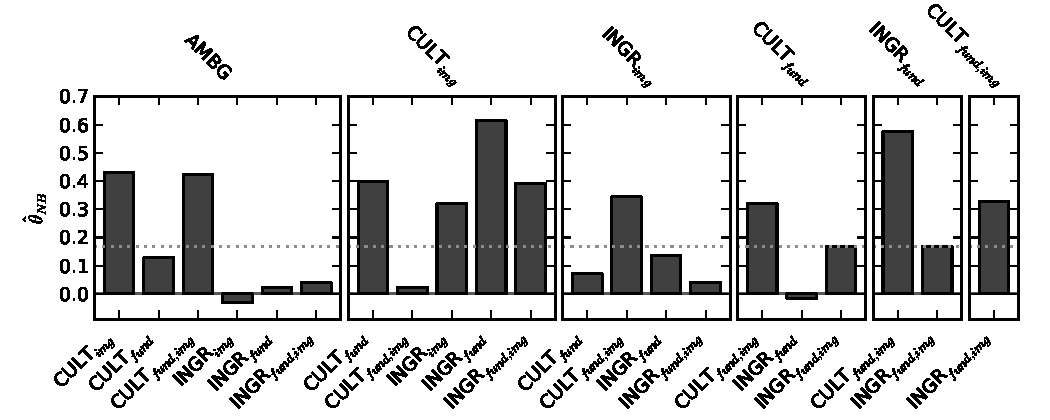
\includegraphics[scale=0.94]{figs/f1-thetas_full_pairwise25_img1.pdf}
	\caption{ \footnotesize{
		Empirical difference in priming, $\hat{\theta}_\text{NB}$, between 
		various treatments.  The difference in priming between each pair of 
		treatments 
		was determined by cross-validation of a Naive Bayes classifier trained
		to classify workers based on the labels they attributed to the first
		image of the final image set. Each panel compares a basis treatment,
		indicated above the panel, to various treatments indicated on the
		abscissa.  We can conclude, with 95\% confidence, that the classifier
		is performing better than chance when $\hat{\theta}_\text{NB}$ 
		exceeds 0.168, indicated by the dotted line.  See \textbf{Methods} for
		the calculation of this confidence threshold.
	}}
\end{figure}

\paragraph{Earlier tasks orient workers' focus during later tasks.} 
We next investigated the \textit{nature} of the inter-task effects.  Since the
initial images were chosen to emphasize either food (ingredients set) or 
culture (cultural set), we looked for effects in the number of culture- and 
food-oriented labels that workers attributed to the final image set.

To this end, we constructed an ontology of labels attributed to the final 
images.  The ontology was constructed as a directed acyclic graph, with edges 
pointing from more general labels to more specific ones.
For example, our ontology contains the path \texttt{food} $\to$ 
\texttt{ingredients} $\to$ \texttt{vegetables} $\to$ \texttt{tomato}. We 
provide more detail about the construction of the ontology in the 
\textbf{Materials and Methods} section.

We counted labels as being culture- and/or food-oriented based on 
whether the label had inbound paths from the abstract labels \texttt{culture} 
or \texttt{food} in the ontology. Since food is a central feature 
of culture, there were many labels that were both culture- and food-oriented 
in this sense.  Nevertheless, there were many food-oriented labels, such as 
\texttt{bread}, which lacked specific cultural connections.  Meanwhile, there 
were many non-food, culture-oriented labels, such as \texttt{russian dolls}. 

When we tallied labels attributed to the first image of the final set, 
we found that workers shown the cultural initial set produced significantly 
more culture-oriented labels and less food-oriented ones 
(see \textbf{Fig. 2A}).  In fact, the inter-task
effect was so strong that it essentially reversed the proportion of culture- 
and food-oriented labels seen for the ambiguous set.  On the other hand, the 
composition of labels attributed by 
workers shown the ingredients image set was not significantly different from 
that attributed by workers shown the ambiguous set.  This shows that inter-task
effects can profoundly alter workers' focus, but the effects brought 
about by showing workers the ambiguous and ingredients sets were not 
significantly different.



\paragraph{Earlier tasks influenced workers' level of specificity.} 
\begin{figure}
	\begin{center}
		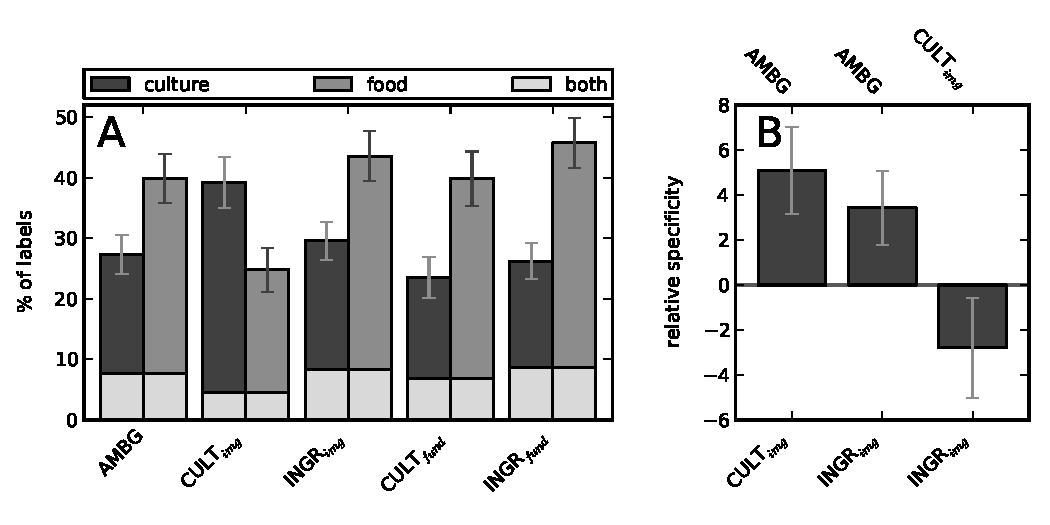
\includegraphics[scale=0.70]{figs/orientation_specificity.pdf}
	\caption{\footnotesize{
		\textbf{A}) Percent label composition (culture- vs food-oriented 
		labels) for 
		various images and treatments.  
		\textbf{B}) Relative specificities of treatments
		indicated along the abscissa compared to those indicated above the 
		plot.  The size of the bar indicates how much more specific
		the labels from one treatment are compared to the other, and points 
		toward in the direction of the more specific treatment.
	}}
	\end{center}
\end{figure}

Using the ontology described in the previous section, we compared treatments 
in their degree of specificity.  When comparing two labels $\ell_1$ and 
$\ell_2$ produced by different workers, we say that $\ell_2$ is more specific 
than $\ell_1$ if there is a \textit{directed path} from $\ell_1$ to $\ell_2$.  
If there is no directed path between $\ell_1$ and $\ell_2$, then they are 
non-comparable.  As an example, \texttt{tomato} is more specific than 
\texttt{food}, while \texttt{statue} and \texttt{food} are non-comparable.

We can compare the degree of specificity of two workers by comparing the 
labels each gives to some image in the final set.  Thus, we define the relative
specificity of worker $u$ and $v$ for the $i$th image in the final set to be
$s_i(u,v)$:

\begin{align}
	s_i(u,v) = \sum_{\ell \in u(i) } \;
	\sum_{m \in v(i)} 
	\left(\mathbf{1}_{[\ell > m]} - \mathbf{1}_{[m>\ell]}\right),
	\label{eq:worker-specificity}
\end{align}

where $u(i)$ denotes the set of labels attributed by worker $u$ to image $i$, 
and $\mathbf{1}_{[\ell > m]}$ evaluates to 1 if $\ell$ is more specific than 
$m$, and 0 otherwise.

We can then define the relative specificity of treatments $\mathcal{U}$ and 
$\mathcal{V}$, with regard to
the $i$th image, $S_i(\mathcal{U},\mathcal{V})$, to be the mean
relative specificity of two workers drawn uniformly from the treatments.  
We obtain the estimator, $\hat{S}_i(\mathcal{U},\mathcal{V})$, by computing
the sample average for our experimental data:

\begin{align}
	\hat{S}_i(\mathcal{U},\mathcal{V}) = 
	\frac{1}{|\mathcal{U}| |\mathcal{V}|}
	\sum_{u \in \mathcal{U}} \;
	\sum_{v \in \mathcal{V}} \;
		s_i(u,v).
		\label{eq:specificity}
\end{align}

Further details for the estimation of relative specificity and the standard
error of the estimation are given in \textbf{Methods}.

We found that, with regard to labels attributed to the first image of the 
final set, workers from \textsc{AMBG} were more specific than workers from
either $\textsc{CULT}_{img}$ or $\textsc{INGR}_{img}$.  When we compare 
$\textsc{CULT}_{img}$ to $\textsc{INGR}_{img}$, we found that workers from
$\textsc{INGR}_{img}$ were more specific.  This shows that inter-task 
effects substantially influence the specificity of labels that workers provide.

\paragraph{Inter-task effects ``wash out'' quickly.}  
\begin{figure}
	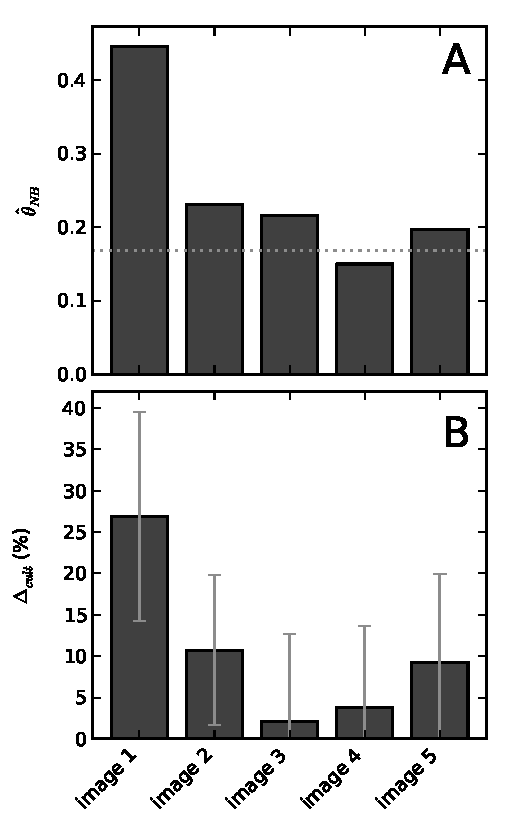
\includegraphics[scale=0.7]{figs/longitudinal_theta_excess-culture.pdf}
	\caption{\footnotesize{
		\textbf{A}) Difference in priming between \textsc{AMBG} and 
		$\textsc{CULT}_{img}$ measured based on the accuracy of a Naive Bayes 
		classifier during cross-validation, when trained on labels from the
		test images indicated along the abscissa.
		\textbf{B}) Excess cultural orientation of labels attributed to
		the test images indicated on the abscissa, by workers from
		$\textsc{CULT}_{img}$ relative to those attributed by workers from
		\textsc{AMBG}, calculated using \textbf{Eq. 3}.
	}}
\end{figure}
At this point we have 
investigated the inter-task effects induced on only the first image of the 
final image set.  This is because, as mentioned, the effects are strongest on 
for first image.  We now examine how the inter-task effects vary as workers 
proceed through the images in the final set.  Since the final images are the
same for all treatments, it would stand to reason that the inter-task effects
induced by the initial image sets would fade away, being washed out by the
inter-task effects of the final set.

Looking at the classifier performance, $\hat{\theta}_{NB}$, with respect to the
treatments \textsc{AMBG} and $\textsc{CULT}_{img}$, we find that performance
drops off dramatically after just the first image (see \textbf{Fig. 3A}).
This suggests that inter-task effects mainly arise between consecutive tasks.
However, a residual distinguishability between these two treatments does 
persist until the final image (although for the fourth image we cannot assert
this with 95\% confidence).

We can similarly look at how the inter-task effects on label composition
(i.e. fraction of culture- and food-oriented words) play out as workers 
progress through the final image set.  To do this, we define the 
\textit{excess cultural orientation} as the number of culture-oriented labels 
minus the number of food oriented ones.  Tracking the excess cultural 
orientation across the images is, however, not in itself meaningful,
because some images will inherently carry more cultural content than others. 
To account for this, we calculate the excess cultural content for both 
\textsc{AMBG} and $\textsc{CULT}_{img}$, and subtract the former from the 
latter, yielding the \textit{relative} excess cultural content, 
$\Delta_{cult}$.  Formally,

\begin{align}
	\Delta_{cult}(i) = \frac{1}{N}\left[ \sum_{w\in\textsc{cult}_{img}} \left(N_{w,cult}^{(i)} - N_{w,food}^{(i)}\right)
	- \sum_{w\in\textsc{ambg}} \left(N_{w,cult}^{(i)} - N_{w,food}^{(i)}\right)\right],
\end{align}

where $N_{w,cult}^{(i)}$ stands for the number of culture-oriented labels 
attributed by worker $w$ to image $i$, while $N_{w,food}^{(i)}$ similarly 
counts food-oriented labels, and $N$ is the total number of labels in a 
treatment.  

The relative excess cultural content varied as workers proceed through the
final image set in much the same way that $\hat{\theta}_\text{NB}$ did: for the
first test image, it is significantly greater than zero, but drops off rapidly
thereafter.  Unlike $\hat{\theta}_\text{NB}$, $\Delta_{cult}$ ceases to
be significantly greater than zero after the second test image, so it would 
seem that $\hat{\theta}_\text{NB}$ is the more sensitive of the two in
detecting inter-task effects.

\paragraph{Inter-task similarity encourages more specific labels.}
For the next part of the analysis, it will be useful to speak of the
``similarity'' between two image sets. In general, the characterization of 
image content 
is deeply complex and has been approached from the perspectives of 
art\cite{panofsky1939studies,shatford1986analyzing},
psychology\cite{Tversky1977327}, and information retrieval\cite{Jaimes20002}.
Furthermore, the perception of \textit{similarity} is a particularly subtle 
psychological phenomenon.  For example, a figure $A$ can appear simultaneously
both \textit{more} and \textit{less} similar to an object $C$ than some other 
object $B$[***].    

In the present study, we are more interested in the ultimate outputs of 
workers' rather than the psychological details which lead to them (though 
these are interesting in their own right).  This allows us to sidestep the 
complication in attributing similarity: we asses how similar two sets of 
images are, 
\textit{with respect to the labeling task}, by looking at the fraction of 
labels that they share.  Formally, we compute the similarity of two images
sets $X$ and $Y$ by computing the Jacquard index between the sets of labels 
attributed to them:

\begin{align}
	\text{Sim}(X,Y) = \frac{L(X) \cap L(Y)}{L(X) \cup L(Y)},
\end{align}

\begin{table}
\centering
\begin{tabular}{ l  d  s s s s}

\toprule    
\multirow{2}{*}{Image set} & \multicolumn{1}{c}{\# of unique} & 
\multicolumn{4}{c}{Similarity}  \\
\cline{3-6}


&  \multicolumn{1}{c}{labels} 
& \multicolumn{1}{c}{Ambiguous} 
& \multicolumn{1}{c}{Cultural} 
& \multicolumn{1}{c}{Ingredients}
& \multicolumn{1}{c}{Test} \\
  
\midrule

Ambiguous & 763 & 1 & 0.0418 & 0.142 & 0.167 \\

Cultural & 659 & 0.0418  & 1 & 0.0347 & 0.0561 \\

Ingredients & 681 & 0.142  & 0.0347 & 1 & 0.110 \\

Test & 1695 & 0.167  & 0.0561 & 0.110 & 1
\\
\bottomrule

\end{tabular}
\caption{\footnotesize{
	Number of unique labels attributed to each image set, and their
	similarities based on \textbf{Eq. 4} 
}}
\label{table:2}
\end{table}

where $L(X)$ denotes the set of labels attributed to $X$.  See \textbf{Methods}
for additional details regarding the calculation of similarity.

The similarities of the various image sets are presented in \textbf{Table 2}. 
First, observe that the ambiguous and ingredients sets are much more similar 
to each other than either is to the culture set.  This is consistent with our
finding that $\hat{\theta}_\text{NB}$ between \textsc{AMBG} and 
$\textsc{INGR}_{img}$ was not significant (see \textbf{Fig 1}).

Next we draw attention to the similarity between the initial sets and the test 
set.  The ambiguous set is the most similar to the test set, followed by the
ingredients set, and the cultural set was most different from the test set.
Observe that these levels of similarity mirror the label specificity for the 
corresponding treatments (c.f. \textbf{Fig. 2B}).  

This suggests that labeling a series of images that are similar to 
one another might encourage workers to use more specific terminology.
Such a phenomenon would be consistent with the psychological mechanism known 
as \textit{negative priming}.  Negative priming occurs when a person becomes 
desensitized to non-salient stimuli to which she is repeatedly 
exposed [***].  Consider that workers who initially 
labeled the ambiguous image set had already seen five images showing 
prepared meals once they labeled the first test image.  At that point,
a worker might not regard the labels \texttt{food} or \texttt{meal} to be 
salient, since they do not distinguish the image from those she had seen 
already.

We are suggesting that, although workers are not instructed to compare
images in any way, prior tasks nevertheless create a frame of reference
relative to which later tasks are judged.  This in turn 
influences the perception of salience. Thus, in a series of subjective 
characterization tasks that have very similar content, the worker's focus 
will tend to be directed away from generic, shared attributes, towards those 
attributes that are specific and distinguishing.


\subsection*{Discussion}

\paragraph{Inter-task effects should be considered during task design.}  
Our results show that inter-task effects can have a strong influence on how
workers label images.  In particular, we observed that prior tasks influence
the specificity and content of labels.  Surprisingly, framing a task by 
indicating a semantically-loaded funder had much milder effects on worker 
outputs, generally below the statistical power of our tests.

We therefore caution those designing studies using human computation: even if 
the requester has eliminated surrounding influences to every practical extent, 
\textit{the greatest source of bias might lurk in the tasks themselves}.
Due consideration should be given to how tasks are bundled together.
While our measurements of $\hat{\theta}_\text{NB}$ indicated that inter-task 
effects persisted even to the fifth test image, the most severe effects arise 
between consecutive tasks.

\paragraph{$\theta$ provides a general purpose measure of priming effects.}
When used three approaches to detecting priming effects: 1) using a Naive Bayes
classifier to measure $\hat{\theta}_\text{NB}$, 2) tallying the number of 
culture- and food-oriented labels, and 3) comparing the relative specificity
of labels based on an ontology.  Of the three, measuring $
\hat{\theta}_\text{NB}$ was the most sensitive.  

In one sense, this is not surprising because the Naive 
Bayes classifier takes into account the frequency of occurrence of all labels 
encountered during training.  But it is remarkable that the 
method which incorporates neither prior knowledge about the image contents nor 
label semantics, outperforms those that do.  This is a powerful feature 
because, given the outputs from two sets of workers, one can test whether they 
have been differently primed without knowing how that priming might manifest.

Our algorithmic definition of priming is phrased in terms of worker outputs
rather than psychological phenomena.  This provides a connection between
the priming effects and their potential to impact decisions made on the basis
of worker outputs.  In the case of a binary decision, $\theta$
describes the worst-case bias introduced by failing to control for priming 
effects.

\paragraph{Batching tasks for better HPU performance.}
Our proposed connection between similarity and specificity during 
image-labeling might be used to tune the specificity of labels.  For example,
If one seeks very nuanced labeling, our results suggest that the images 
should first be sorted into batches based on their similarity. This could be 
accomplished by beginning with a first, coarse characterization of unsorted 
images, followed by batching based on the labels obtained. Then, the batches
of similar images could be served for a second round of finer labeling. 
The sorting and re-labeling could then in principle be repeated.

In effect, this creates a hierarchical workflow, where the first, 
coarsely-characterizing HPUs provide a stream of labeled images that is 
split (batched) and fed to other HPUs for finer characterization.  This 
workflow exhibits an interesting difference between HPUs and CPUs.  In general,
whenever an aspect of a problem can be parallelized when employing CPUs, one
gains efficiency.  But here, because of HPU hysteresis, we see an example where
one might sacrifice accuracy through parallelization.

\subsection*{Conclusion}


Inter-task priming can have a strong effect.  
For a canonical image-labeling task, inter-task priming was stronger in its 
effects on the orientation and specificity of labels than was the disclosure of
semantically loaded funder names.  Requesters on microtask platforms should 
take care to avoid introducing biases due to the batching and ordering tasks 
they serve to workers.  At the same time, inter-task priming might be exploited to improve task output, for 
example, to drive more (or less) nuanced responses.

We demonstrated that our algorithmic definition of priming, and its 
implementation using a Naive Bayes classifier, provides a sensitive,
general-purpose method for detecting priming.  Even when the expected effects 
on label orientation and specificity were slight, $\theta_\text{NB}$ 
was significant.  $\theta_\text{NB}$ provides direct statistical evidence that 
populations have been affected by priming, even when the nature of the 
effects are not understood. 

\subsection*{Materials and Methods}

\textbf{AMT Tasks.} The task described in \textbf{Experimental Setup}
was served to 900 workers, who were uniformly randomly assigned to
treatments.  Each treatment had at least 126 task completions.  To obtain 
uniformly sized treatments, we randomly selected 126 samples from each 
treatment. Workers were
only allowed to participate once and could not see the initial or final 
images, nor the funder names when previewing the task.

\textbf{Naive Bayes Classifier.}
The features provided to the Naive Bayes classifier consisted of the labels
that the worker provided along with the image and specific location in which 
the label was entered
(each image had five distinct label inputs).  Thus, \texttt{wine} occurring in 
position 1 of image 2 would be considered as a distinct feature from 
\texttt{wine} occurring in position 2 of image 2. The classifier 
had better performance when this distinction was made.

\textbf{Building the ontology of terms.}  The ontology was built manually
by the experimenters, starting from the corpus of labels. Labels occurring only 
once were discarded.  We created the root classes \texttt{activity}, 
\texttt{adjective}, \texttt{culture}, 
\texttt{food}, and \texttt{thing}. \texttt{culture} and \texttt{food} were 
given top-level status because they were prominently represented in the corpus.
Whenever one label was judged to be a more specific case of another, a
directed edge was drawn from the more general to the more specific. This
judgment call was made by the experimenters.  However, the labels from all 
treatments were aggregated before assembling the ontology,  to 
ensure that the ontology construction would not be affected by 
knowledge of the treatments from which labels originated. 
Labels which were judged to be roughly synonymous were treated as identical,
and labels judged to be misspellings were corrected. 

\textbf{Statistical significance of $\theta_\text{NB}$.}
We test the significance two population's measured $\theta_\text{NB}$ against 
the null hypothesis that that the two populations are in fact identical:
\begin{align}
	\mathbf{H_0}: \theta_\text{NB} = 0 \\
	\mathbf{H_1}: \theta_\text{NB} > 0
\end{align}
If the populations are in fact identical, then the probability that the 
classifier correctly classifies a worker is $\frac{1}{2}$. Let $K$ be a random
variable which denotes the number of correct classifications when the 
classifier is challenged to classify a total of $n$ workers during 
cross-validation.  Under $\mathbf{H_0}$, the probability distribution of $K$ 
is:
\begin{align}
	\text{Pr}\{K = k | n \} = { n \choose k } \left(\frac{1}{2}\right)^n.
\end{align}
We can reject $\mathbf{H_0}$ at significance $\alpha$ if $\theta_\text{NB}$ 
is greater than or equal to a critical value, $\theta_\text{NB}^*$:
\begin{align}
	\theta^*_\text{NB} = \frac{2k^*}{n} - 1
\end{align}
where $k^*$ is the smallest integer in $\{0,\dots,n\}$ that satisfies 
\begin{align}
	\sum_{k \in \{k^*, \dots, n\}} \text{Pr}\{K = k | n \} < \alpha.
\end{align}
For a 5-fold cross-validation with non-overlapping test sets containing 25 
workers ($n = 125$), and a significance of $\alpha = 0.05$, we
have $k^*=73 \implies \theta_\text{NB}^* = 0.168$.






\textbf{Statistical significance of relative specificity.}
We used \textbf{Eq.~\ref{eq:specificity}} to compute the relative specificity
of two treatments.  To analyze relative specificity statistically,
we first develop \textbf{Eq.~\ref{eq:specificity}} from an intermediate 
definition.  Let the specificity of a worker $u$ relative to a 
\textit{basis treatment} $\mathcal{V}$, denoted $S_V(u)$, be the expected 
relative specificity between $u$ and a worker uniformly sampled from 
$\mathcal{V}$:

\begin{align}
	S_V(u) =  \text{E}_V\{s(u,V)\}, \quad V \in_R \mathcal{V},
		\label{eq:basis-specificity}
\end{align}
where $V$ is a random, uniformly sampled worker from $\mathcal{V}$.  We 
subscript the expectation operator with $V$ to indicate 
that the expectation is taken over the distribution of $V$.  Then, the 
relative specificity of two treatments, $S(\mathcal{U},{V})$, can be 
written as:
\begin{align}
	S(\mathcal{U},\mathcal{V}) = 
		\text{E}_U\{S_V(U)\}, \quad U \in_R \mathcal{U},
		\label{eq:treatment-specificity}
\end{align}
where $U$ is a random, uniformly sampled worker from $\mathcal{U}$.  This 
yields 
estimators for $S_V(u)$ and $S(\mathcal{U}, \mathcal{V})$, and their variances
as shown below (note that 
\textbf{Eq.~\ref{eq:treatment-specificity-estimator}} is
equivalent to \textbf{Eq.~\ref{eq:specificity}}):

\begin{align}
	\hat{S}_V(u) &= \frac{1}{|\mathcal{V}|} \sum_{v \in \mathcal{V}} s(u,v), 
		\label{eq:basis-specificity-estimator} \\
		\hat{S}(\mathcal{U},\mathcal{V}) 
		&= \frac{1}{|\mathcal{U}|} \sum_{u \in \mathcal{V}} \hat{S}_V(u),
		\label{eq:treatment-specificity-estimator} \\
		\text{Var}_V\{\hat{S}_V(u)\} 
			&= \frac{1}{|\mathcal{V}|}\text{Var}_V\{s(u,V)\},
		\label{eq:basis-specificity-variance} \\
		\text{Var}_{U,V}\{\hat{S}(\mathcal{U},\mathcal{V})\} 
			&= \frac{1}{|\mathcal{V}|\cdot|\mathcal{U}|^2} 
			\sum_{u\in U}\text{Var}_V\{{s}(u,V)\}.
		\label{eq:treatment-specificity-variance}
\end{align}
\td{There are problems with this.  I'm still trying to figure out how to
	calculate the variance properly.}
$\text{Var}_V\{s(u,V)\}$ can be directly calculated as a sample variance.
\textbf{Equations \ref{eq:basis-specificity-estimator}} through 
\textbf{\ref{eq:treatment-specificity-variance}} provide enough information to test the hypotheses:
\begin{align}
	\begin{matrix}
		\mathbf{H_0}: S(\mathcal{U}, \mathcal{V}) = 0 \\[0.5em]
		\mathbf{H_1}: S(\mathcal{U}, \mathcal{V}) \neq 0
	\end{matrix}
\end{align}

\begin{figure}
	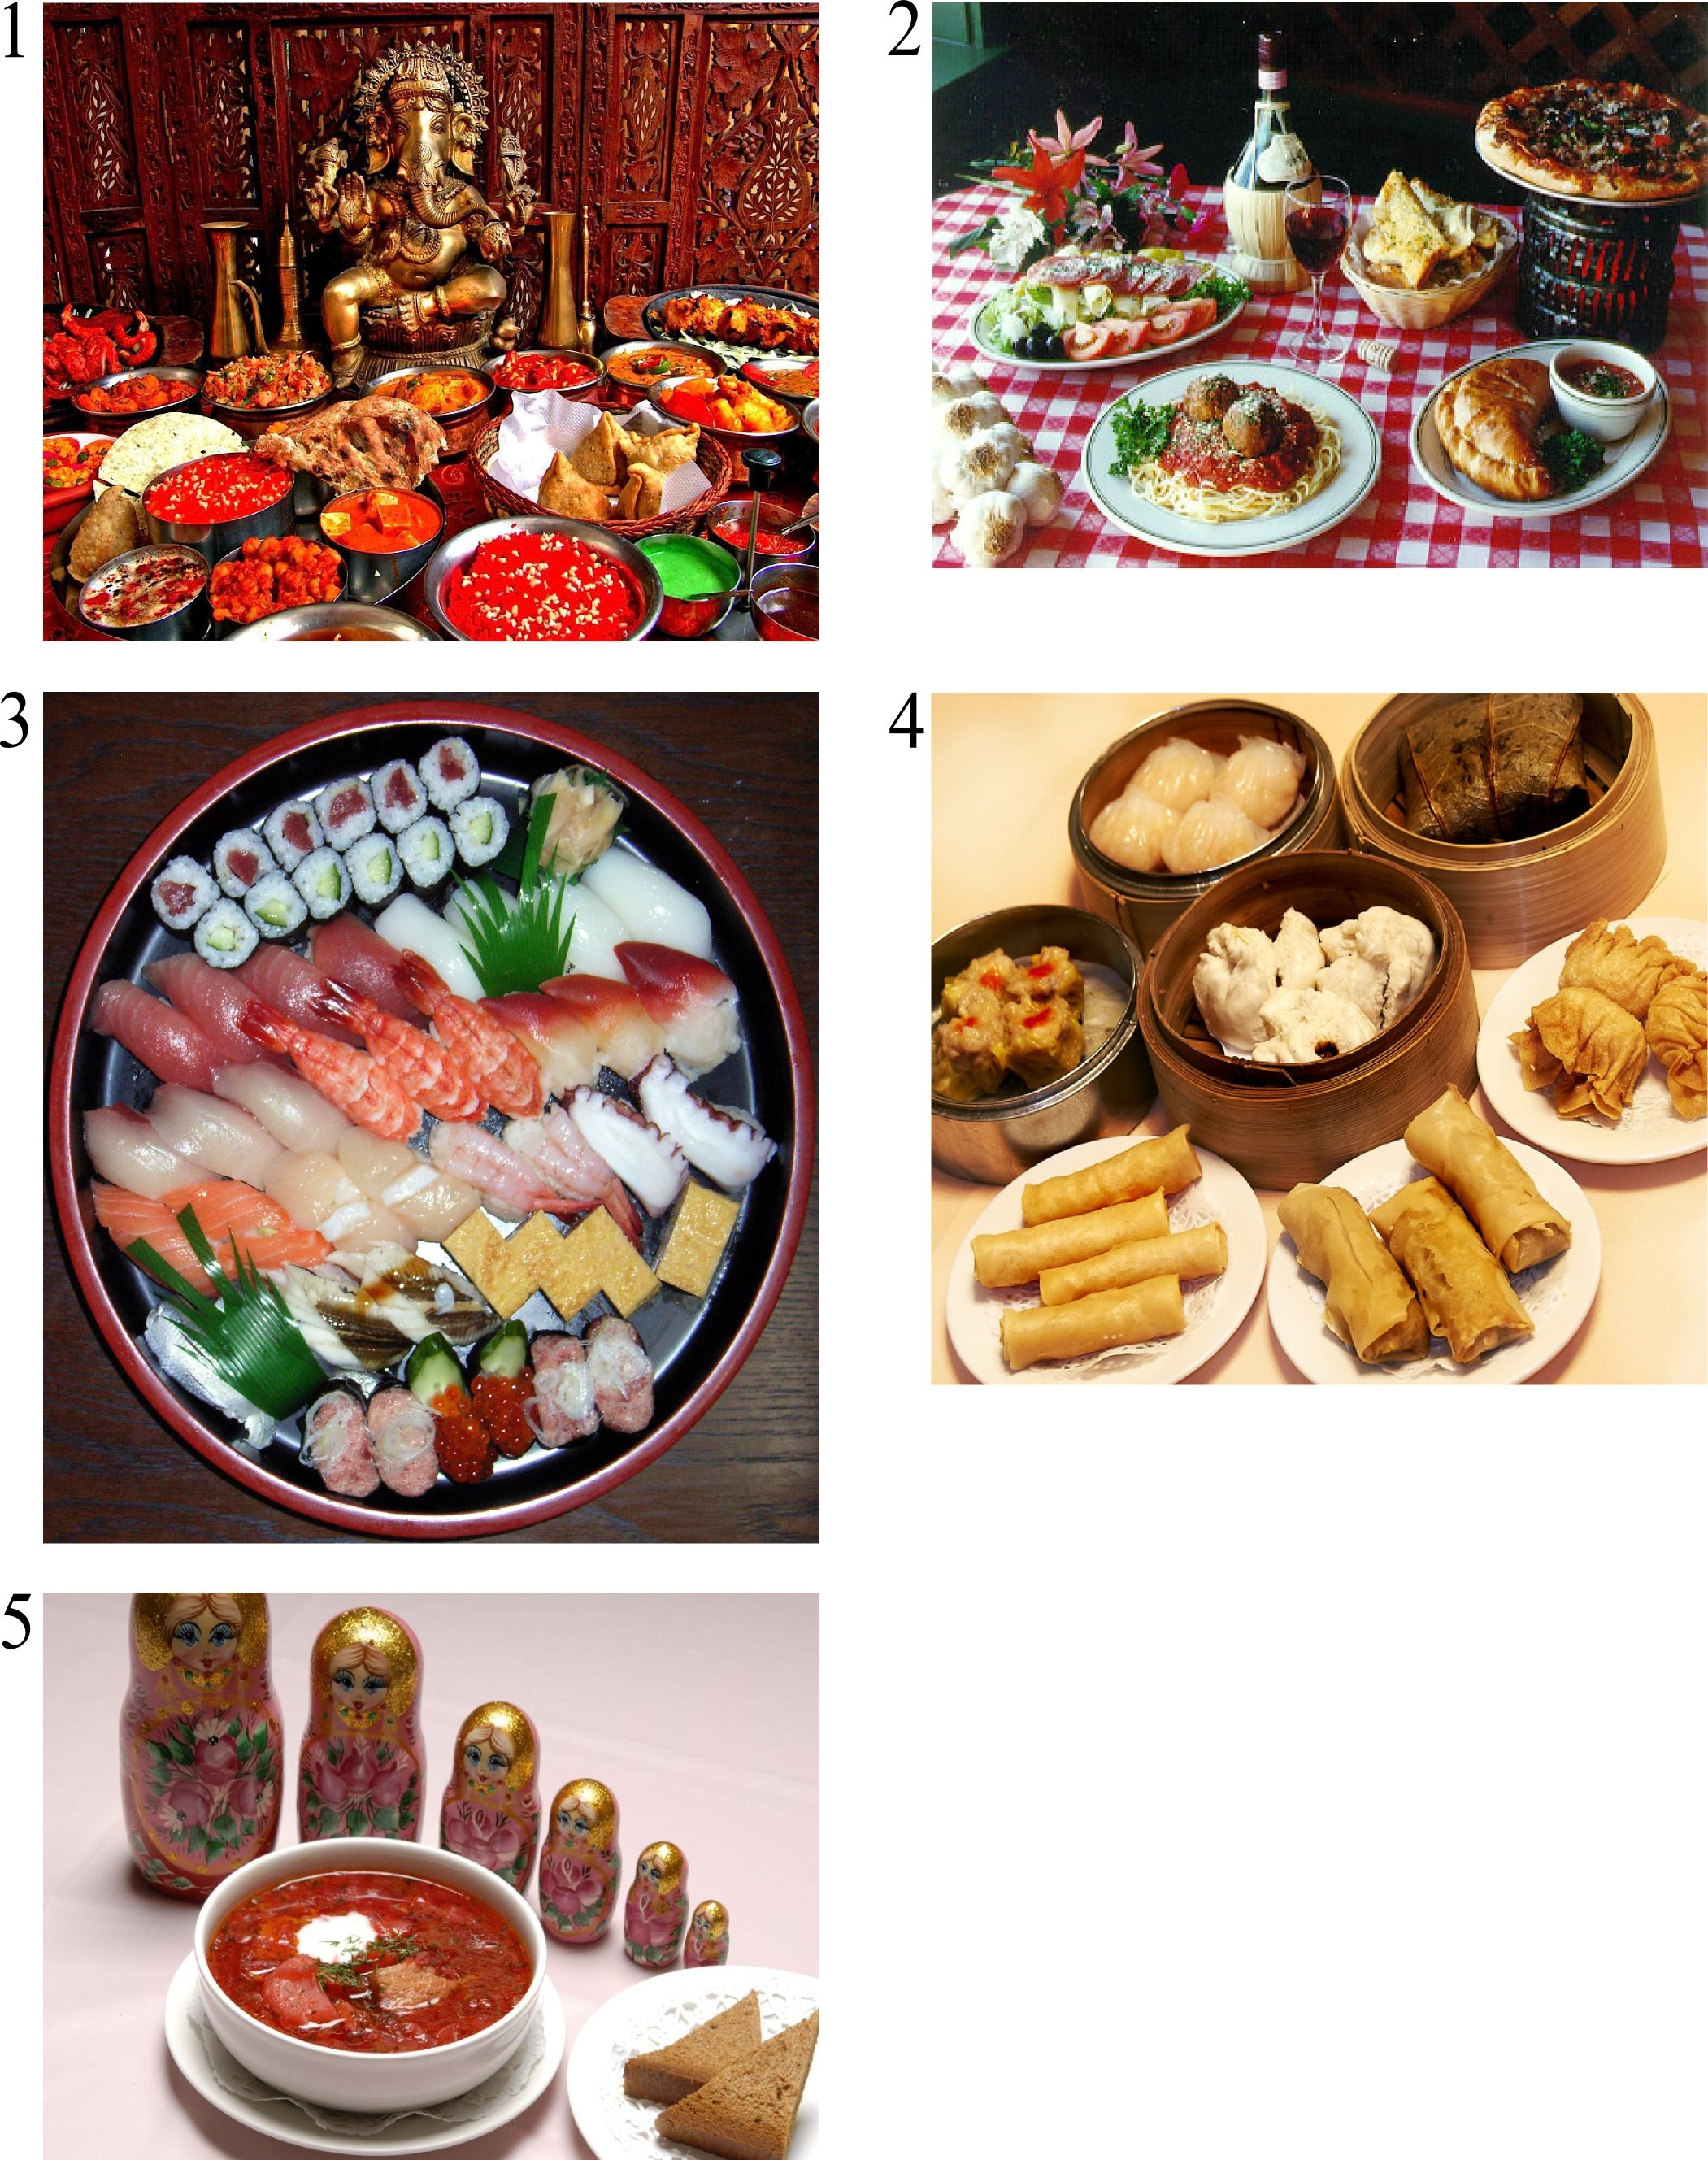
\includegraphics[scale=1.00]{figs/taskImages/testImages.jpg}
	\caption{Testing image set. These images were presented to all workers in 
		the order shown after the priming set of images.}
\end{figure}

\begin{figure}
	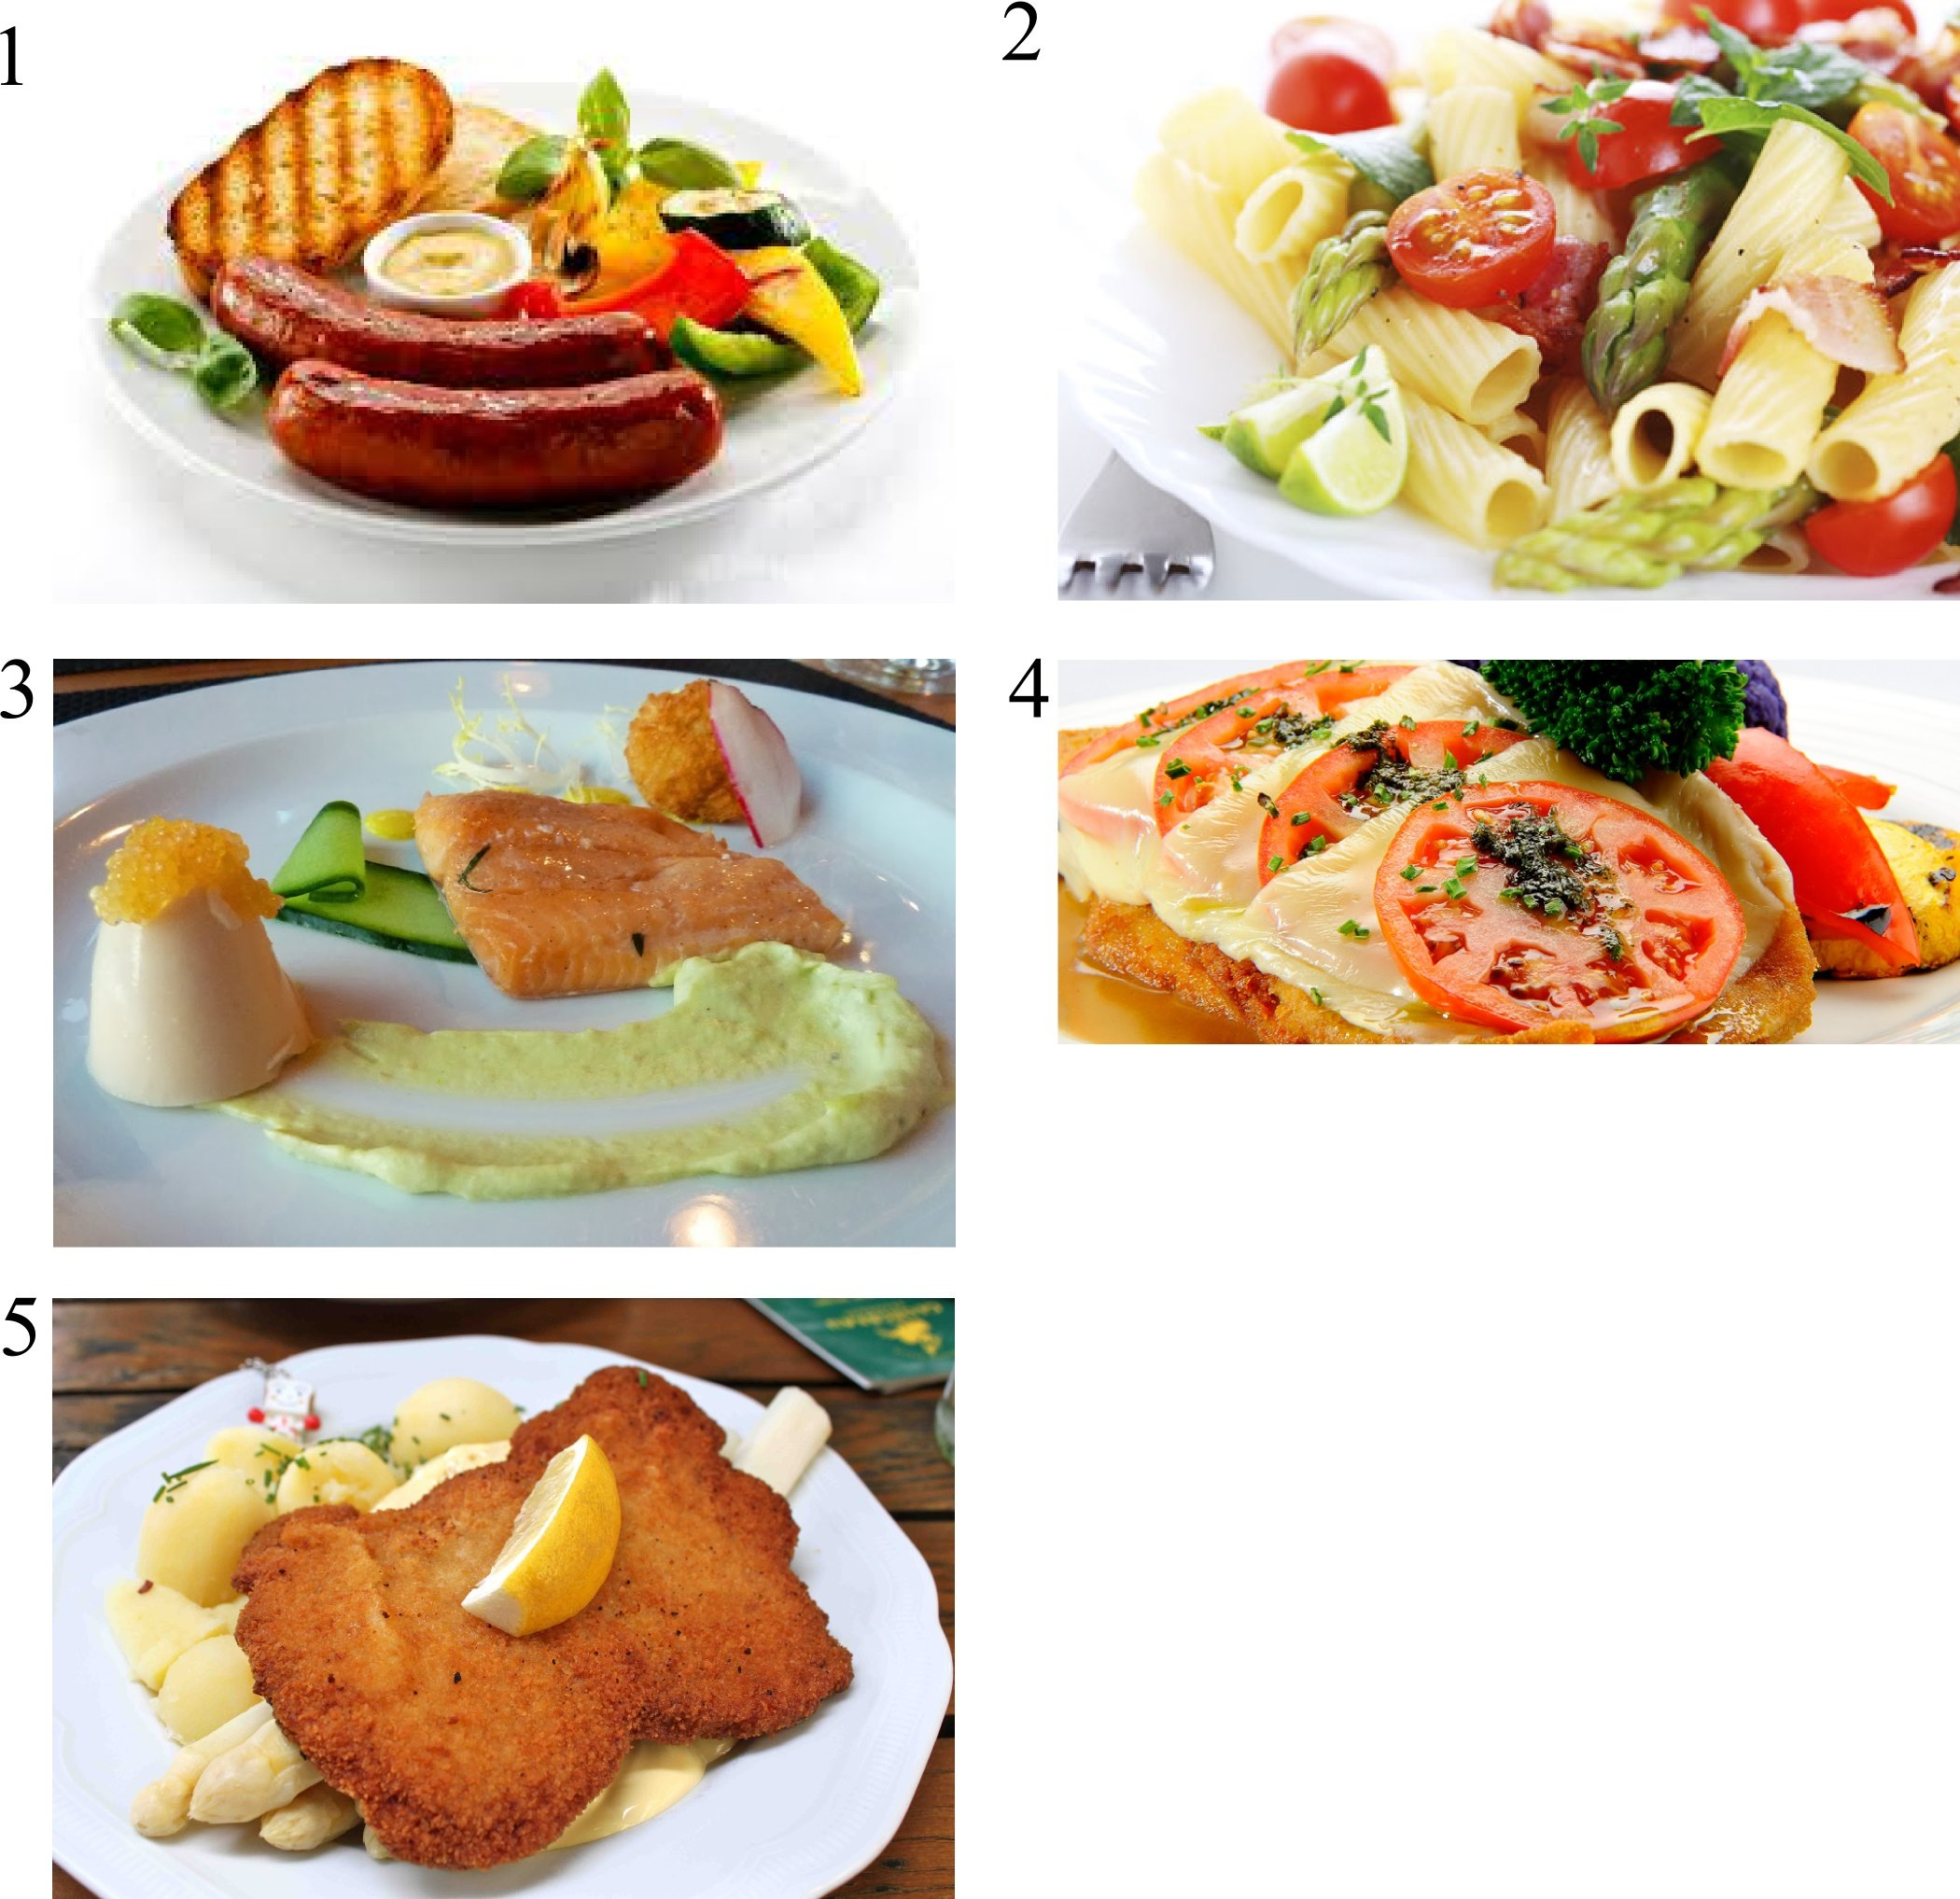
\includegraphics[scale=1.00]{figs/taskImages/ambiguous.jpg}
	\caption{ Ambiguous image set. These images were presented to workers from 
		certain treatments (see \textbf{Table 1}) in the order shown.}
\end{figure}

\begin{figure}
	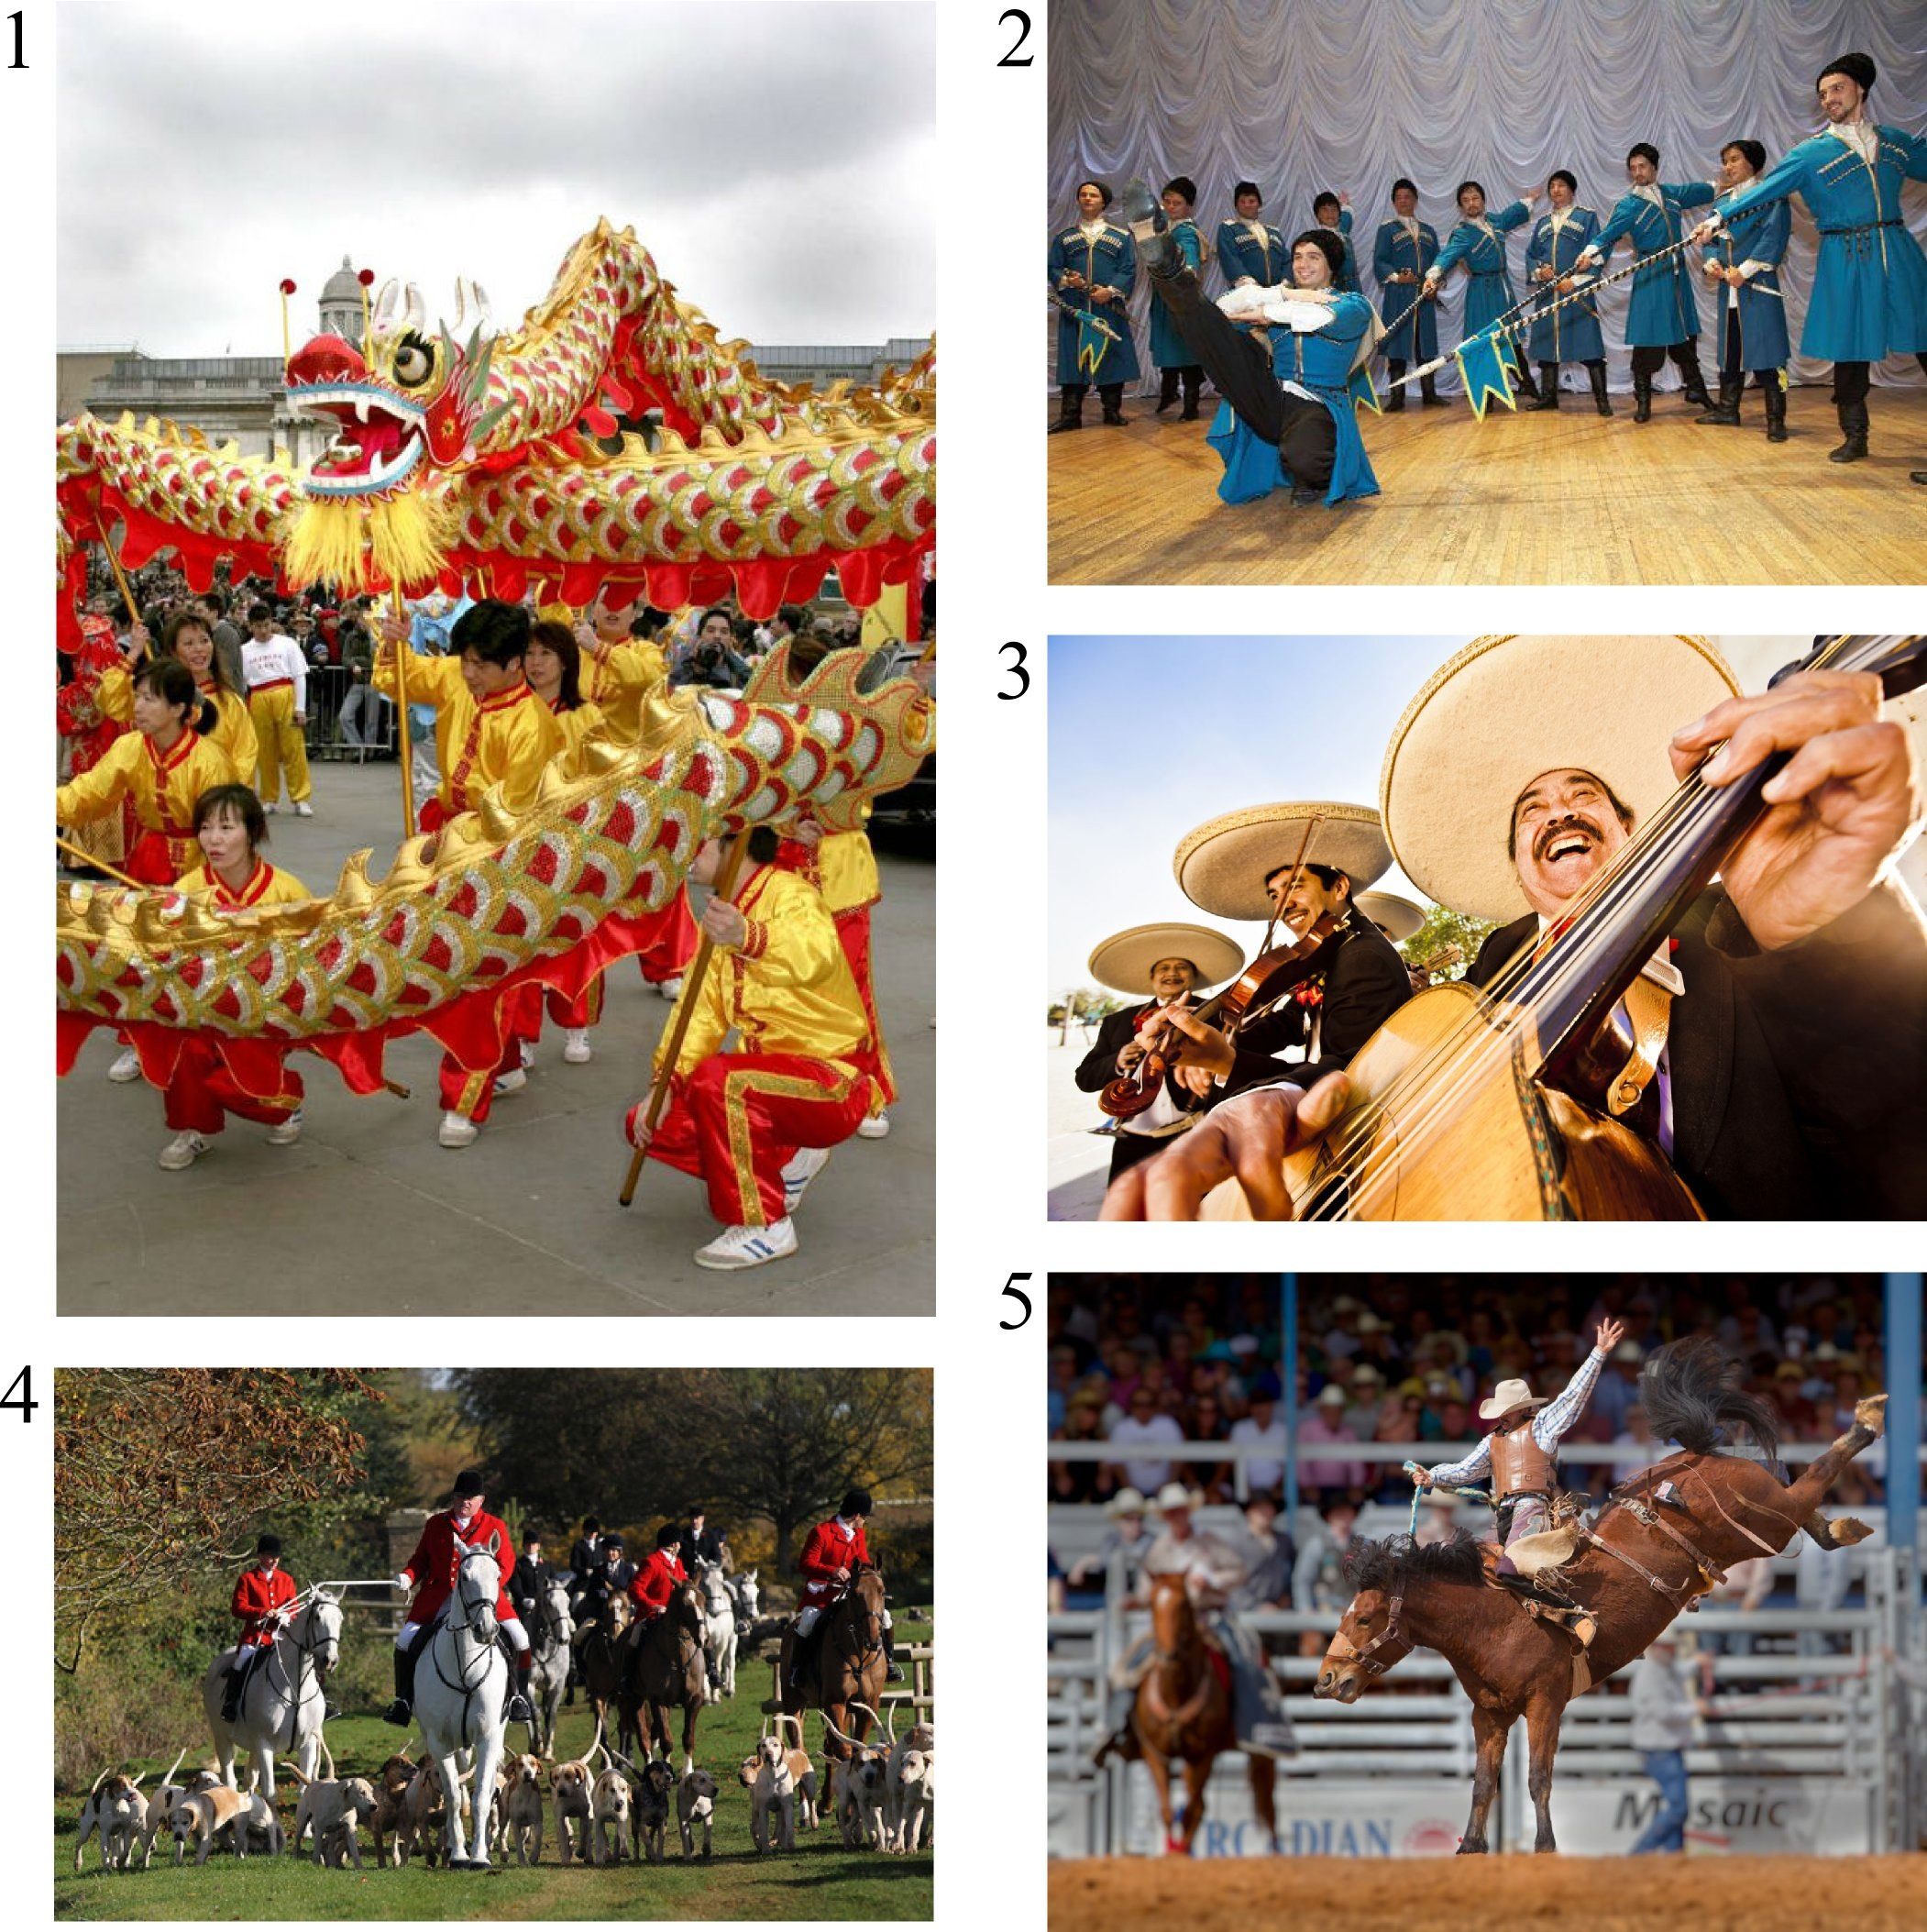
\includegraphics[scale=1.00]{figs/taskImages/cultural.jpg}
	\caption{Cultural image set. These images were presented to workers from 
		certain treatments (see \textbf{Table 1}) in the order shown.}
\end{figure}

\begin{figure}
	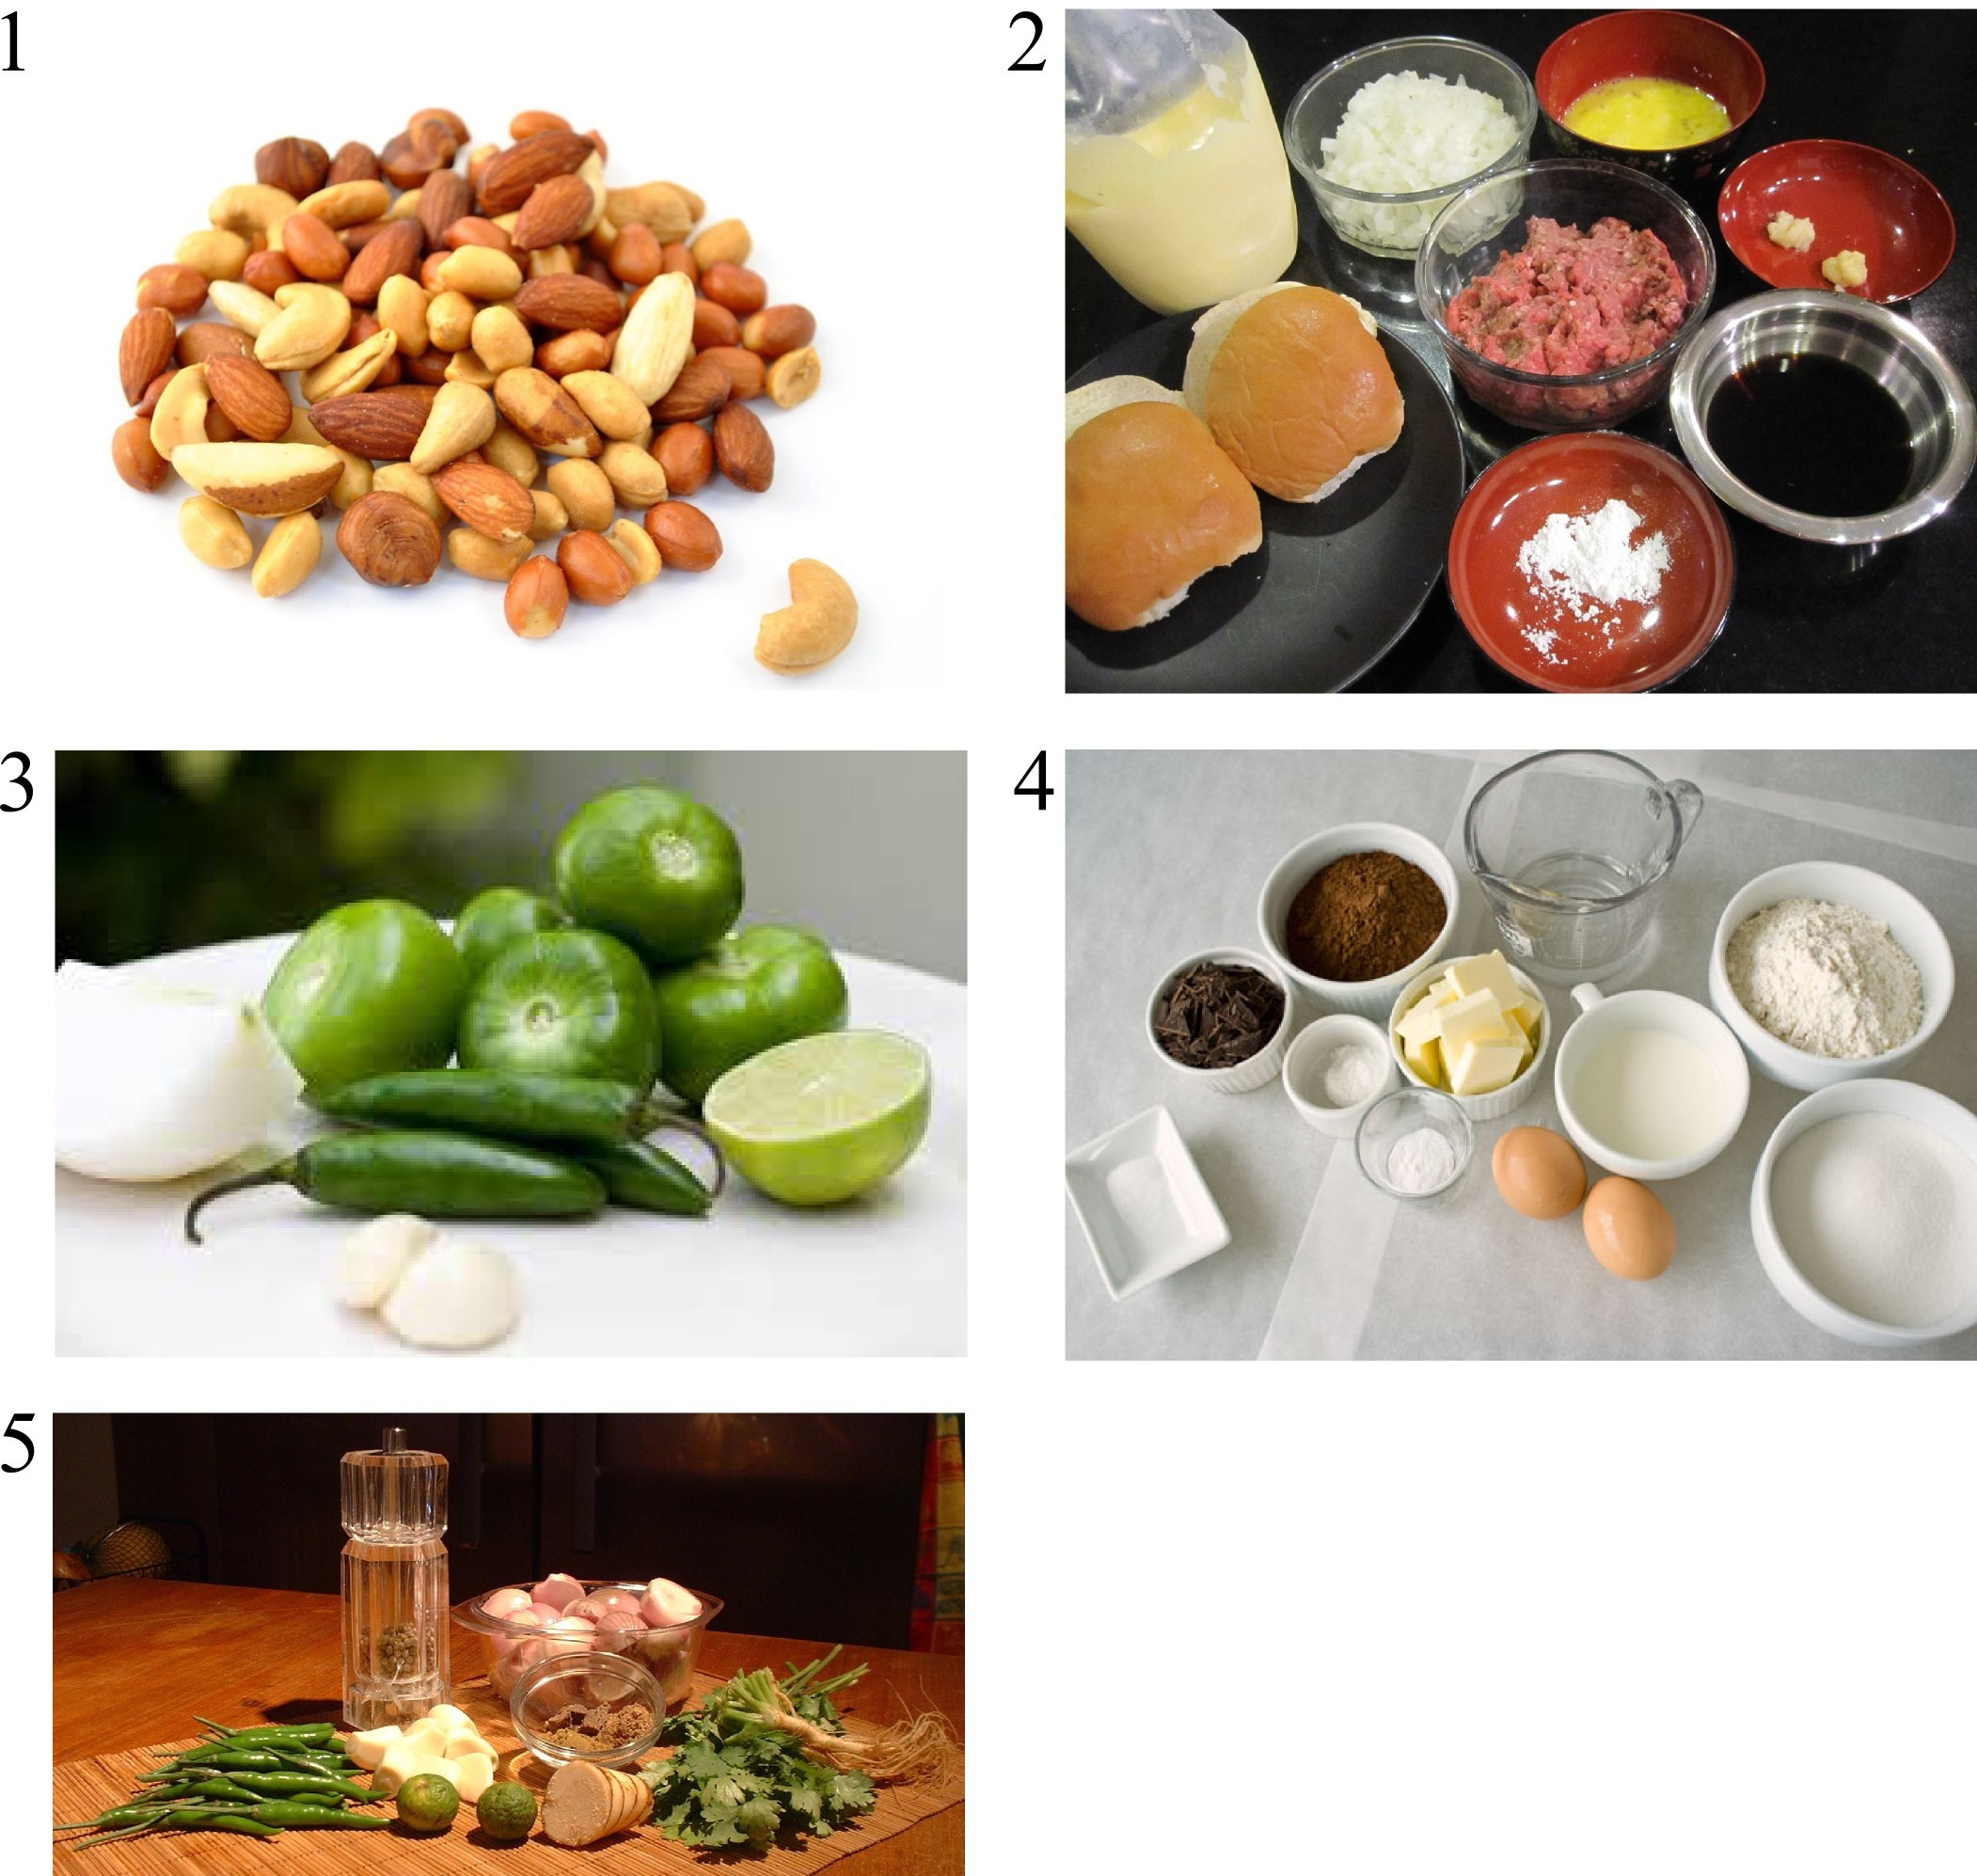
\includegraphics[scale=1.00]{figs/taskImages/ingredients.jpg}
	\caption{ Ingredients image set. These images were presented to workers 
		from certain treatments (see \textbf{Table 1}) in the order shown.}
\end{figure}
\section*{Acknowledgments}
\section*{References}
\begingroup
\renewcommand{\chapter}[2]{}
\bibliography{newbib.bib}
\endgroup
\bibliographystyle{plain} 

\end{document}


